%-------------------------------------------------------------------------------
% Literature review of recent advances in modeling seismic waves propagation using machine   
% learning-based methods
%-------------------------------------------------------------------------------
% Author: oscar-rincon
% Email: orincon@eafit.edu.co
% Creation date: 2024-03-15
% Version: 1.0
%-------------------------------------------------------------------------------
\documentclass[11pt,twoside]{article}
%-------------------------------------------------------------------------------
% Import the style file
%-------------------------------------------------------------------------------
\usepackage{preprint}
\usepackage{lipsum}
% Macro to highlight text that still needs your input
\newcommand{\todo}[1]{\textcolor{red}{[#1]}}
%-------------------------------------------------------------------------------
% Document starts here
%-------------------------------------------------------------------------------
\begin{document}

% Set the page style to empty (no headers or footers)
\thispagestyle{empty}  

%-------------------------------------------------------------------------------
% Title, Author, and Affiliation
%-------------------------------------------------------------------------------

% Create a colored box with specific background and frame colors, and sharp corners
%\begin{tcolorbox}[colback=white!20,colframe=gray!20,sharp corners]

% Add vertical space adjustment
\vspace{-2mm} 
% Create a minipage for the title
\begin{minipage}{15.0cm}
    \begin{center}
        % Title of the document
        \textbf{\large Applications of a Hybrid BEM–PINN Method to Inverse Wave Propagation Problems in Irregular Topographies}  
    \end{center}                 
\end{minipage} 
% Create a minipage for the first logo
\begin{minipage}{0.0cm}
    \begin{center}
        % Include the first logo with specific width
        %\hspace{-0.2cm}\includegraphics[width=2.8cm]{figs/format/eafit.pdf}
    \end{center}
\end{minipage}    
 
% Add vertical space adjustment
\vspace{-2mm} 
%\end{tcolorbox}

% Add vertical space adjustment
\vspace{0.6cm}
 
{\footnotesize\noindent O. Rincón-Cardeño$^1$, S. Montoya-Noguera$^2$, and N. Guarín-Zapata$^{1,*}$ \\
$^1$ Mathematical Applications in Science and Engineering Research Group, School of Applied Sciences and Engineering, Universidad EAFIT, 
  Medellín, Colombia \\
$^2$ Nature and Cities Research Group, School of Applied Sciences and Engineering, Universidad EAFIT, Medellín, Colombia\\
  $^*$ Correspondence: nguarinz@eafit.edu.co}
 
 

%-------------------------------------------------------------------------------
% Abstract of the document
%-------------------------------------------------------------------------------

% Create a colored box with specific background and frame colors, and sharp corners
\begin{tcolorbox}[colback=gray!20, colframe=gray!20, sharp corners]

    % Begin the abstract section
    \begin{abstract}

        % Add vertical space adjustment
        \vspace{-1mm}

        % No indentation for the first paragraph
        \noindent
        % Abstract content      
\noindent Topographic irregularities affect seismic ground motion. Predicting these effects requires knowledge of subsurface geometry and material properties, which are often unavailable at field scale and must be inferred from seismic records. This leads to ill-posed inverse problems. The boundary element method (BEM) is well suited to wave propagation in semi-infinite domains, while physics-informed neural networks (PINNs) offer advantages for inverse parameter estimation through automatic differentiation. However, BEM-based inversion requires repeated forward solutions, whereas PINNs face challenges in representing wave radiation in unbounded domains. In this work, we investigate the application of a hybrid BEM–PINN approach to inverse seismic problems in irregular topographies. Three scenarios are considered: identification of the hill–half-space interface, reconstruction of the free-surface geometry, and joint estimation of geometry and material properties.\\
    \end{abstract}
\end{tcolorbox} 

\noindent\textbf{Keywords:} Boundary element method; physics-informed neural networks; inverse problems; topographic effects; wave scattering


 
%-------------------------------------------------------------------------------
% Section - Introduction
%-------------------------------------------------------------------------------
\section*{Introduction}\label{sec:introduction}
\fancyhead[RO]{\textit{Introduction}\, / \thepage}
%-------------------------------------------------------------------------------

\lettrine[lines=2,loversize=0.15,findent=0.4em,nindent=0em]{\textcolor{gray}{T}}{}opographic irregularities such as hills, ridges and canyons modify seismic ground motion, producing amplification and deamplification patterns that depend on surface geometry, subsurface structure and wave incidence angle \citep{Bard1982,Kawase1988}. Predicting these effects requires knowledge of the geometry and material properties of the medium, which are often uncertain or unavailable at field scale. Consequently, these parameters must be inferred from seismic records, leading to inverse problems involving geometric and material identification.

The boundary element method (BEM) is well suited to wave propagation in semi-infinite domains because it discretizes only boundaries and interfaces and naturally satisfies the radiation condition through appropriate Green's functions. Previous studies have used BEM to identify buried interfaces from surface-wave records \citep{Bignardi2012}, reconstruct free-surface geometries from scattering data \citep{Wang2018}, and jointly estimate the shape and material properties of elastic inclusions \citep{Bonnet2009}. However, BEM-based inversion relies on repeated forward solutions, making the optimization computationally demanding and potentially sensitive to noise and initial estimates \citep{Kallivokas2009,Chien2005}. Physics-informed neural networks (PINNs) offer an alternative for inverse parameter estimation by treating unknown quantities as trainable variables and computing derivatives through automatic differentiation \citep{Raissi2019}. They have been applied to wave propagation in anisotropic media and irregular topographies \citep{Song2022}, as well as full waveform inversion \citep{RashtBehesht2022}. However, accurately representing wave radiation in unbounded domains remains challenging. These complementary capabilities motivate the combination of physics-based numerical methods with machine learning to address problems that are challenging for either approach alone. In this context, hybrid BEM–PINN approaches have been explored in electromagnetics \citep{Barmada2024} and SH-wave scattering by complex topographies \citep{wu_novel_2026}. Although these studies demonstrate the potential of such combinations for forward wave propagation, their application to geometric and material inversion in seismic topographies remains unexplored.

In this work, we investigate the application of a hybrid BEM–PINN approach to three inverse seismic problems: (i) identification of the buried interface between a hill or sedimentary deposit and the underlying half-space, assuming known material properties; (ii) reconstruction of the free-surface geometry from scattering data; and (iii) joint identification of geometry and material properties. The motivation is to combine the capabilities of BEM for representing wave propagation in semi-infinite domains with the trainable parameter estimation capabilities of PINNs. Through these applications, we evaluate the suitability of this combination for inverse seismic characterization, considering reconstruction accuracy, sensitivity to measurement noise, and the influence of receiver locations, frequencies and wave incidence angles.

\section{Geometric and Material Inversion in Irregular Topographies}\label{sec:problem_statement}

We consider the inverse characterization of an irregular topographic feature
overlying a semi-infinite elastic half-space. Seismic responses are assumed
to be available at a set of observation points under prescribed wave
excitation conditions. The objective is to estimate unknown geometric and
material parameters by comparing observed responses with those predicted by
the forward wave propagation model. Three inverse problem configurations
are considered, as illustrated in Fig.~\ref{fig:problem_statement}.

\begin{figure*}[ht!]
    \centering
    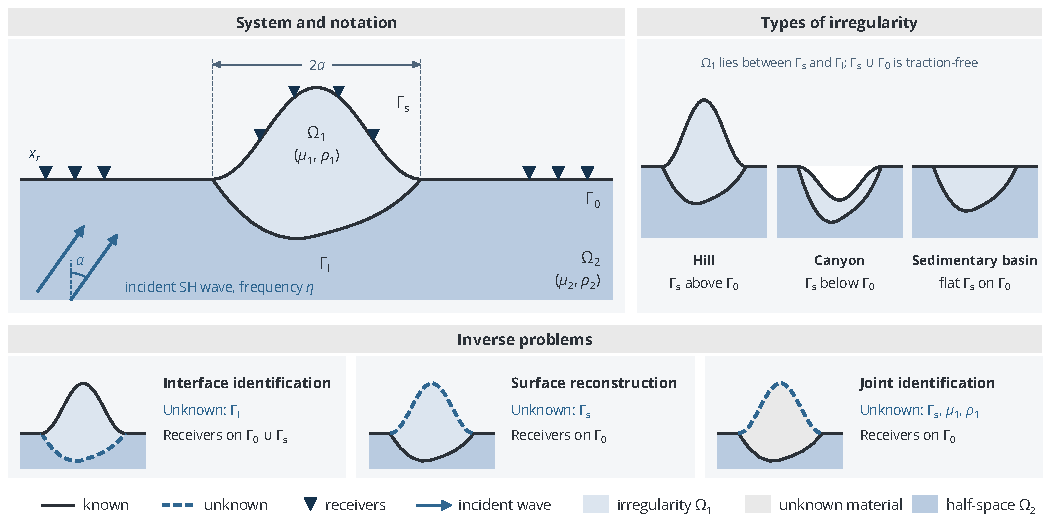
\includegraphics[width=6.5in]{figures/problem_statement.pdf}
\caption{Problem setting. Top left: an irregularity $\Omega_1$ with properties
  $(\mu_1,\rho_1)$, bounded by the free surface $\Gamma_s$ and the interface
  $\Gamma_I$, embedded in a half-space $\Omega_2$ with properties $(\mu_2,\rho_2)$
  and flat free surface $\Gamma_0$, excited by a plane SH wave with frequency
  $\eta$ and incidence angle $\alpha$; receivers $\mathbf{x}_r$ are placed on
  $\Gamma_0$ and, when it is known, on $\Gamma_s$. Top right: types of
  irregularity considered. Bottom: inverse problems; dashed orange lines and
  orange shading denote unknowns, and all other quantities are known.}
    \label{fig:problem_statement}
\end{figure*}



\noindent\textbf{Buried-interface identification.} The free-surface geometry and material properties of the hill and underlying half-space are assumed known, while the geometry of the interface separating the two media is unknown. Its reconstruction from seismic observations provides information about the subsurface structure without requiring direct access to the contact between the two media.\\

\noindent\textbf{Free-surface reconstruction.} The buried interface and material properties are assumed known, while the external topographic profile is unknown. The objective is to recover the free-surface geometry from the seismic response, accounting for the effects of surface irregularities on wave scattering.\\

\noindent\textbf{Joint geometry and material identification.} Both the geometry and material properties of the hill are unknown and must be estimated simultaneously from the seismic observations. This introduces additional complexity because geometric and material variations can produce similar effects on the wavefield, potentially increasing the non-uniqueness of the inverse problem.

\section{Hybrid BEM--PINN Inversion}\label{sec:methodology}

The inversion strategy extends the BEM--PINN formulation of \citet{wu_novel_2026}
from forward scattering to geometric and material identification. A neural
network represents the source densities of an indirect boundary element
formulation, so the governing equation and the radiation condition are satisfied
exactly by construction, while the boundary conditions and the seismic records
enter as penalties in a single loss function. The geometric and material
unknowns are treated as additional trainable variables and are updated jointly
with the network weights (Fig.~\ref{fig:methodology_scheme}).

\begin{figure*}[ht!]
    \centering
    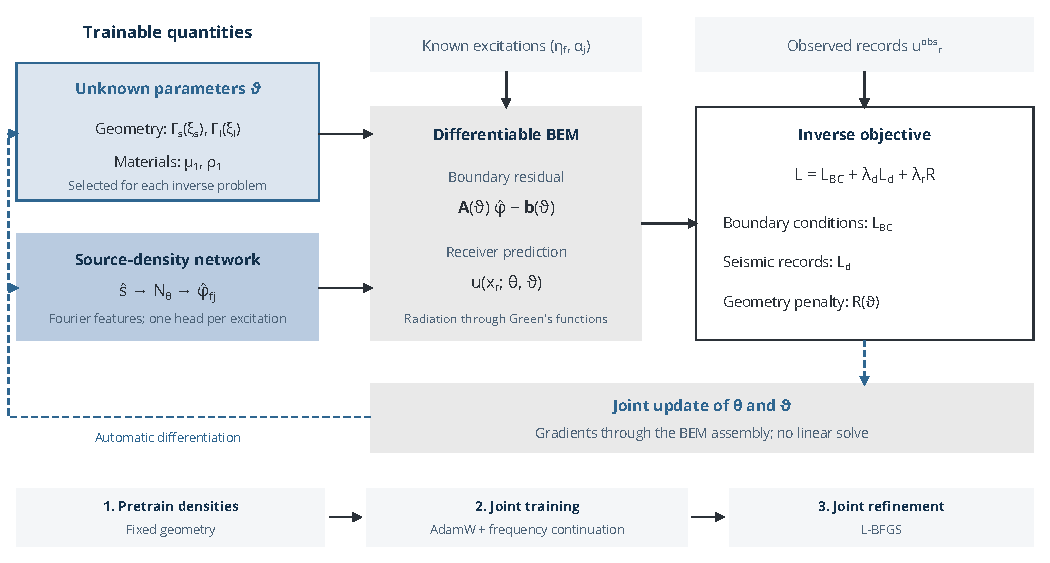
\includegraphics[width=6.5in]{figures/methodology_scheme.pdf}
    \caption{Hybrid BEM--PINN inversion scheme. A fully connected network with
      Fourier-feature inputs maps the boundary coordinate $s$, the normalized
      frequency $\eta$ and the incidence angle $\alpha$ to the source densities
      of the indirect BEM. The BEM representation gives the boundary-condition
      residuals at the collocation points $\mathbf{x}_n$ and the predicted
      response at the receivers $\mathbf{x}_r$. The network weights $\theta$
      and the unknowns $\vartheta$ (orange) are updated jointly by minimizing
      $L(\theta,\vartheta)$.}
    \label{fig:methodology_scheme}
\end{figure*}

 

We consider antiplane (SH) motion with time dependence $e^{i\omega t}$. The hill
$\Omega_1$, with shear modulus $\mu_1$ and density $\rho_1$, is bounded by the free
surface $\Gamma_s$ and the interface $\Gamma_I$. It overlies the half-space
$\Omega_2$, with properties $(\mu_2,\rho_2)$, whose flat free surface outside the
hill is $\Gamma_0$. The out-of-plane displacement $u_j$ in $\Omega_j$ satisfies
\begin{equation}
  \nabla^2 u_j + k_j^2 u_j = 0 \quad \text{in } \Omega_j,
  \qquad k_j = \frac{\omega}{\beta_j},\quad \beta_j = \sqrt{\mu_j/\rho_j},
  \qquad j = 1,2,
\end{equation}
subject to
\begin{equation}\label{eq:bcs}
  t_1 = 0 \ \text{on } \Gamma_s, \qquad
  t_2 = 0 \ \text{on } \Gamma_0, \qquad
  u_1 = u_2,\ \ t_1 = t_2 \ \text{on } \Gamma_I,
\end{equation}
where $t_j = \mu_j\,\partial u_j/\partial n$ is the traction and $\mathbf{n}$ on
$\Gamma_I$ points from $\Omega_1$ into $\Omega_2$. The excitation is a plane SH
wave with incidence angle $\alpha$ and normalized frequency
$\eta = \omega a/(\pi\beta_2)$, where $a$ is the half-width of the hill. Following the indirect BEM \citep{SanchezSesma1991,wu_novel_2026}, each field
is written as a single-layer potential:

\begin{align}
  u_1(\mathbf{x}) &= \int_{\Gamma_s\cup\Gamma_I}
     \phi^{(1)}(\mathbf{x}_0)\, G_1(\mathbf{x},\mathbf{x}_0)\, dS(\mathbf{x}_0),
     & \mathbf{x}&\in\Omega_1, \label{eq:u1}\\
  u_2(\mathbf{x}) &= u^{f\!f}(\mathbf{x}) + \int_{\Gamma_I}
     \phi^{(2)}(\mathbf{x}_0)\, G_2(\mathbf{x},\mathbf{x}_0)\, dS(\mathbf{x}_0),
     & \mathbf{x}&\in\Omega_2. \label{eq:u2}
\end{align}
Here $G_1 = \frac{1}{4i\mu_1}H_0^{(2)}(k_1 r)$ is the full-space Green's function,
$G_2$ is the half-space Green's function obtained by adding the image source
with respect to $\Gamma_0$, so that $t_2=0$ on $\Gamma_0$ holds identically, and
$u^{f\!f}$ is the free-field response of the flat half-space (incident plus
reflected plane waves). Both representations satisfy the Helmholtz equation, and
the scattered part of $u_2$ satisfies the Sommerfeld radiation condition, so
the remaining conditions in~\eqref{eq:bcs} are those on $\Gamma_s$ and $\Gamma_I$. The boundaries are divided into $N_e$ elements $\Delta S_l$ with centers
$\mathbf{x}_{0,l}$, which serve as both source and collocation points. With a
constant density per element,

\begin{equation}\label{eq:discrete}
  \begin{gathered}
  u_1(\mathbf{x}) = \sum_{l} \hat\phi^{(1)}_l\, G_{1,l}(\mathbf{x}),\qquad
  u_2(\mathbf{x}) = u^{f\!f}(\mathbf{x}) + \sum_{l} \hat\phi^{(2)}_l\, G_{2,l}(\mathbf{x}),\\
  G_{j,l}(\mathbf{x}) = \int_{\Delta S_l} G_j(\mathbf{x},\mathbf{x}_0)\, dS(\mathbf{x}_0),
  \end{gathered}
\end{equation}
and the tractions follow by differentiating $G_{j,l}$ along $\mathbf{n}$. The
integrals are computed by Gaussian quadrature. On the self-element, the
logarithmic singularity of $G_j$ is integrated analytically and the traction
receives the free term $\pm\tfrac12\hat\phi_l$ \citep{SanchezSesma1991}. Rather than solving the linear system implied by~\eqref{eq:bcs}
and~\eqref{eq:discrete}, the densities are represented by a fully connected
network $\mathcal{N}_\theta$. Its input is $\mathbf{z} = (s,\eta,\alpha)$, where
$s\in[0,1]$ is a curve coordinate shared by $\Gamma_s$ and $\Gamma_I$. Its
output is the real and imaginary parts of the three densities:

\begin{equation}
  \bigl(\hat\phi_s,\ \hat\phi_I^{(1)},\ \hat\phi_I^{(2)}\bigr)(\mathbf{z})
  = \mathcal{N}_\theta\bigl(\gamma(\mathbf{z})\bigr),
  \qquad
  \gamma(\mathbf{z}) = \bigl[\sin(2\pi\mathbf{B}\mathbf{z}),\ \cos(2\pi\mathbf{B}\mathbf{z})\bigr],
\end{equation}
where $\hat\phi_s$ and $\hat\phi_I^{(1)}$ are the restrictions of
$\hat\phi^{(1)}$ to $\Gamma_s$ and $\Gamma_I$, and $\hat\phi_I^{(2)}$ is the
density radiating into $\Omega_2$. The Fourier feature mapping $\gamma$, with a
random matrix $\mathbf{B}\in\mathbb{R}^{m\times 3}$, reduces the spectral bias
of the network toward low-frequency functions \citep{Tancik2020}. This is needed
because the densities oscillate faster as $\eta$ increases. The hidden layers
are $\mathbf{h}^l = \sigma(\mathbf{W}^l\mathbf{h}^{l-1} + \mathbf{b}^l)$, with
trainable parameters $\theta = \{\mathbf{W}^l,\mathbf{b}^l\}$. Parametrizing the
densities by $s$ instead of by Cartesian coordinates keeps the network input
fixed while the geometry evolves during inversion.

\subsection{Parametrization of the unknowns}

Both curves share the end points $x=\pm a$ and are written as
\begin{equation}\label{eq:shape}
  \Gamma_s:\ \bigl(x,\ y\bigr) = \Bigl(a(2s-1),\ \sum_{k=1}^{K}\xi_{s,k}\sin(k\pi s)\Bigr),
  \qquad
  \Gamma_I:\ \bigl(x,\ y\bigr) = \Bigl(a(2s-1),\ -\sum_{k=1}^{K}\xi_{I,k}\sin(k\pi s)\Bigr),
\end{equation}
so a truncated sine series with coefficients
$\boldsymbol{\xi}_s,\boldsymbol{\xi}_I\in\mathbb{R}^K$ determines the geometry.
The vector of unknowns $\vartheta$ depends on the configuration in
Fig.~\ref{fig:problem_statement}:
(i)~$\vartheta = \boldsymbol{\xi}_I$;
(ii)~$\vartheta = \boldsymbol{\xi}_s$;
(iii)~$\vartheta = (\boldsymbol{\xi}_s,\mu_1,\rho_1)$.
All other quantities are fixed at their known values. The material parameters
are optimized in logarithmic form to keep them positive. The source points
$\mathbf{x}_{0,l}(\vartheta)$, collocation points $\mathbf{x}_n(\vartheta)$,
normals, element lengths and wavenumber $k_1(\mu_1,\rho_1)$ all depend
differentiably on $\vartheta$.

\subsection{Loss function and joint optimization}

For a batch of frequencies and incidence angles, the boundary conditions on
$\Gamma_s$ and $\Gamma_I$ are imposed at the collocation points:
\begin{equation}
  L_{BC} = \bigl\langle |t_1|^2 \bigr\rangle_{\Gamma_s}
  + \bigl\langle |u_1-u_2|^2 \bigr\rangle_{\Gamma_I}
  + \bigl\langle |t_1-t_2|^2 \bigr\rangle_{\Gamma_I},
\end{equation}
where $\langle\cdot\rangle_{\Gamma}$ is the mean over the collocation points on
$\Gamma$ and over the $(\eta,\alpha)$ samples. Displacements and tractions are
nondimensionalized by the free-field amplitude and by $\mu_2 k_2$, respectively.
The seismic records $u^{obs}_r = u^{obs}(\mathbf{x}_r;\eta,\alpha)$ at the
receivers $\mathbf{x}_r\in\Gamma_0$ enter through
\begin{equation}
  L_d = \bigl\langle |u_2(\mathbf{x}_r) - u^{obs}_r|^2 \bigr\rangle,
  \qquad
  R(\vartheta) = \sum_{k=1}^{K} k^{2p}\bigl(\xi_{s,k}^2 + \xi_{I,k}^2\bigr),
\end{equation}
where $R$ is a Sobolev-type penalty that favors smooth geometries and limits the
non-uniqueness of the problem. The total loss is
\begin{equation}\label{eq:loss}
  L(\theta,\vartheta) = L_{BC} + \lambda_d L_d + \lambda_r R(\vartheta),
\end{equation}
and the network weights and the unknowns are updated jointly,
\begin{equation}
  \theta^{k+1} = \theta^k - \zeta\,\nabla_\theta L, \qquad
  \vartheta^{k+1} = \vartheta^k - \zeta\,\nabla_\vartheta L,
\end{equation}
using Adam followed by L-BFGS. Automatic differentiation gives
$\nabla_\vartheta L$ through $k_1$ and through the kernels
$G_j(\mathbf{x}_n(\vartheta),\mathbf{x}_{0,l}(\vartheta))$, so no shape
derivatives or adjoint problems need to be derived. Unlike classical
BEM-based inversion, the forward problem is not solved again at every iteration:
the forward and inverse problems converge simultaneously. Training proceeds in three stages. (1)~With $\vartheta$ fixed at an initial
guess $\vartheta^0$, the network is pretrained on $L_{BC}$ alone, which amounts
to a forward BEM solution. (2)~$\vartheta$ is released and~\eqref{eq:loss} is
minimized, starting from the lowest frequencies and adding higher ones
progressively, so that the misfit does not become trapped in local minima.
(3)~L-BFGS refines the result.

 
%-------------------------------------------------------------------------------
% Import references from the bibliography file
%-------------------------------------------------------------------------------
\bibliography{refs}

\end{document}
%-------------------------------------------------------------------------------
% Document finish here
%-------------------------------------------------------------------------------